\documentclass[12pt]{article}
\usepackage{amsmath}
\usepackage[pdftex]{graphicx}
\usepackage{natbib}
\usepackage[margin=1in]{geometry}

\title{Community ecology on isolated islands: Macroecology meets
  evolution}

\author{
  first: A. J. Rominger, K. Goodman, J. Lim and F. Valdovinos, \\
  all others, \\
  last: R. G. Gillespie, D. S. Gruner, George Roderick
}

\date{}

%%%%%%%%%%%%%%%%% END OF PREAMBLE %%%%%%%%%%%%%%%%

\begin{document}
\baselineskip24pt
\maketitle 
\clearpage

\section*{Abstract}
\paragraph{Aim.}
Islands are bedrock model systems in the development of ecological and
evolutionary theory. The Hawaiian Islands in particular have expanded
our understanding of island biogeography, with phylogeographic studies
of rapid diversification and the dynamics of adaptive radiation
overlaid upon a detailed understanding of ecosystem development and
senescence. These studies demonstrate the overriding importance of in
situ speciation in biodiversity patterns of highly isolated
archipelagoes, beyond the reach of equilibrium colonization
dynamics. Here, we ask, how do biodiversity and complex ecosystems
emerge from ecological (dispersal, trophic interactions and population
dynamics) and evolutionary (speciation, extinction, adaptation and
genetic structuring) processes? We synthesize these approaches to
understand the processes driving emergent patterns of island
biodiversity. We use the natural experiment provided by the island
chronosequence to develop a novel analytical pipeline that combines
both macroecological (interaction networks and maximum entropy
inference) and evolutionary (population genetics and phylogenetics)
approaches.

\paragraph{Location.}
The Hawaiian Islands.

\paragraph{Methods.}
We examine how populations of arthropods are structured across the
youngest landscapes in order to ascertain processes involved in early
diversification, focusing in particular on potential differences
between trophic levels.  We then construct food webs based on
arthropod taxa found at a given site with substrates ranging 50 years
to 5m years.  These networks' nodes are then compared to those
predicted by a theory of maximum entropy and a model of food-web
dynamics.  These theories lack mechanisms for
diversification. Deviations of data from theory may thus illuminate
mechanisms of differentiation, such as population structure, incipient
speciation, ecological function, and site age in the evolutionary
assembly trophic interaction networks.

\paragraph{Results.}
We show that, based on genetic information, lineages at lower trophic
levels show higher endemism early on in the island
chronosequence. Higher trophic levels also show local endemism, though
it arises more slowly and over larger areas. Moreover, considering
plant-feeding insects only, we found that younger sites were more
nested and less modular than older sites.

\paragraph{Main conclusions.}
The results, although preliminary, highlight the potential of our
approach in terms of understanding the interplay between ecological
and evolutionary processes in the assembly of complex communities.

\section*{Introduction}

%% islands are important because...
Islands have played an important role in understanding many of the
fundamental principles driving patters of biodiversity, from theories
of evolution(Darwin, Wallace) to the ecology of species richness
and abundance in and out of equilibrium \citep{macWilson, brown1995,
  rosindell2011}. The discrete and replicated nature of island systems has
presented scientists with a natural experiment shedding light on
general processes responsible for the generation and maintenance of
biodiversity.

%% evol studies in islands have shown...(foundation of nat select,
%% area effect on speciation, adaptive rad due to various mechanisms,
%% others?)
Understanding evolutionary change over time has generally been studied
in the context of single lineages, prime examples being the adaptive
radiation of Galapagos finches (citation XXX), Anolis lizards in the
Caribbean (citation XXX), and cichlid fish in the great lakes of
Africa (citation XXX). Studies that have examined early stages of
nascent adaptive radiation in single lineages have provided some of
the most important insights into adaptive diversification, although
the conditions involved in the initiation of the diversification
remain unclear. In particular, while competition (Rundle et al. 2003;
Schluter 2003) and predation (Nosil \& Crespi 2006) are implicated in
species formation, diversification is also attributed to a release
from such antagonistic interactions (Gillespie 2009; Yoder et
al. 2010). Moreover, while some studies indicate that diversification
is associated with specialization, others have found that species
diversification is linked to expansion or modification of the resource
base (Schluter 2000; Wellenreuther et al. 2008; Glor 2010). 
%% this works well with noting that Haleakala has increased generality
%% of endemics plus increased modularity because plants diversify

Likewise, given finite ecological opportunity, one argument suggests
that the rate of diversification should decline as species numbers
increase during an adaptive radiation (Harmon et al. 2008; Rabosky \&
Lovette 2008; Bokma 2009); other arguments highlight the importance of
species themselves as a resource base for others, with diversification
increasing with species number (Ehrlich and Raven 1964, niche
construction book, erwin). Clearly, the community context is of
critical importance in the process of diversification.

%% ecol studies in islands have shown...(priority effects,
%% equilibrium, drift)
Considering ecological patterns during a given snapshot in time,
islands systems have been critical in developing our understanding of
the role of stochastic immigration and extinction in structuring local
biodiversity and linking local scale patterns to regional dynamics
(e.g. Hubbell's local and meta communities
\citep{hubbell2001}). Stemming from the success and failure of
Hubbell's stochastically-focused theory, other researchers have
advanced our understanding of the maintenance of biodiversity both
through re-invigorating classical ecological mechanisms, such as niche
partitioning and preemption \citep{chessonAndThem, fukami}, and also
continuing to explore the statistical properties of large ecological
assemblages \citep{ettinneCrew, conlisk, mcgill,
  harte2011}. Concurrently, researchers have combined statistical and
deterministic perspectives to gain insight into the structure and
stability of ecological networks \citep{williams2000, brose2006,
  berlow2009, romanuk2009, harte2011}.

These synthetic theories of biodiversity, at the level of community
composition and interaction networks, promise the distillation of
universal ecological mechanisms from disparate and noisy
data. However, incorporating an evolutionary perspective remains a
challenge and limitation to the scope of insights from these theories
\citep{ricklefs1987, qian2005}.  There is a clear need to advance
these and similar ecological theories from the static to the dynamic,
so as to understand how biodiversity changes during evolutionary
community assembly, via the processes of invasion, extinction, and in
situ diversification. Ecological networks provide a prime starting
place due to the existing body of theories on both the ecological
outcome of complex interactions \citep{williams2000, brose2006} but
also the evolution of mutualism \citep{thompson, others}, plant-animal
and plant-pathogen interactions \citep{jansen, blackRiver, thompson,
  XXXX} and predation \citep{XXXX}.

%% research is needed to link ecol and evol because...
Biodiversity research has progressed tremendously over recent years
\citep{XXXX} following these largely separate trajectories of
lineage-specific evolutionary studies and macroscopic
(i.e. multi-taxon and large spatial/temporal scale) ecological
studies. Merging these two areas of research is key for understanding
the dynamics of biodiversity through space and time, and in light of
environmental change. However, merging theories that gain their
predictive power from large-scale patterns across multiple species
\citep{brown1995, harte2011} with those that yield information on the
dynamic nature of single lineages is not straightforward.  
%% here we do...
%% hypotheses for age-structured landscape
%% hypotheses for continuum of evol <--> ecol
%% hypotheses about ecol/evol feedback
Here, we outline a set of eco-evolutionary hypotheses to confront this
challenge by predicting the structure of biological assemblages along
a continuum of evolutionary assembly to ecological assembly. We show
how the age-structure landscape of the Hawaiian archipelago, and 
similar oceanic island systems, provides an ideal natural experiment
for testing these hypotheses. We compile published data to present a
preliminary exploration of our hypotheses in Hawaii.

\subsection*{Eco-evolutionary hypotheses and age-structured
  landscapes}

Evolution has largely been viewed as the process responsible for
generating diversity while ecology is said to maintain it
\citep{XXXX}. However, it has long been recognized, and recent research
has crystalized the fact, that ecology and evolution feedback on
each other in a dynamic process. Ecology drives evolution by both
providing opportunities for selective differentiation and potentially
imposing limits to invasion of new diversity---either diversity
derived from immigration or {\it in situ}
differentiation/divergence. This can happen through ecological
interactions between species and their biotic and abiotic environments
producing selective pressures, facilitation and/or
competition. Demographic processes (e.g. dispersal, population
fluctuation) can also lead to diversification through fragmentation of
the gene pool.

Age structured landscapes offer multiple snapshots in time after
differing durations of community assembly and evolution. These
``freeze frames'' provide the opportunity to assess if different
ecological pressures become more or less relevant during a lineage's
diversification. For example, demographic stochasticity could be
critical in generating initial barriers to gene flow between young
incipient species that are then further driven apart by differential
selection. Continued selection could then drive species further up
fitness peaks, increasing isolation and governing community dynamics
through the mechanisms of niche differentiation and fitness
differences. Conversely if niches (i.e. position in the adaptive
landscape) differ between species but fitnesses are roughly equal then
diversity will be determined by neutral drift during periods of
abiotic environmental stability and Gleasonian assembly during
environmental change.  Detailed data on population structure and
selection will be needed to test such hypotheses, data that does not
currently exist but which we intend to collect.

The evolutionary context of community assembly is also critical for
understanding spatial patterns in diversity during a snapshot in time
\citep{ricklefs1987, losos2003nature, gillespie2004,
  ecoEvoMinnowGuy}. As evidenced above, the evolutionary history of a
lineage in a given region determines its exploration of its adaptive
landscape, in turn potentially driving the long-term stability and
diversity of the communities it invades \citep{chessonCrew,
  romingerSuperStat}. Evolution can also lead to unique ecological
outcomes if diversification happens coincidentally with ecological
assembly in space and time. Under such a scenario ecology and
evolution could feedback on each other to produce a constantly
shifting biodiversity baseline.

For the history influence we hypothesize...

We hypothesize that the contribution of evolutionary assembly and
ecological assembly will vary between taxa and between ages of
lineages in communities. Specifically we hypothesize that during
periods of ecological assembly, strongly influenced by immigration
communities will statistical assemblages matching expectations of
statistical steady state \citep{harte2011} after primary succession has
completed. Before primary succession has completed such communities
will likely be in transitory states as they progress toward
statistical steady state. We hypothesize that if a lineage experiences
{\it in situ} diversification rapidly enough to keep pace with
ecological processes that the ecological communities they form could
be driven into alternate evolutionary states that fail to meet the
predictions of purely statistical theories that do not account for
evolutionary dynamics.
%% NOTE FOR GRUNER PAPER: Fukami says alternate transitory states
%% should be related to beta-div and we see beta-div correlated with
%% mete

%% other hyp??

%% network hypotheses: modularity from syndromes, nestedness from
%% barrier traits. nestedness could also come from short-term
%% ecological 

[how to test these hypotheses in the context of Hawaii...we want to
actually leave quite a few hypotheses untestable given current data so
we motivate future work]

Two key interlinked types of studies needed for a broad understanding
of biodiversity dynamics are: (i) examination of diversification
across multiple lineages that co-occur across the same dynamic
landscape in order to evaluate systematic differences between lineages
in rates and patterns of diversification; and (ii) measurement of
macroecological metrics within these communities as they have changed
over time in order to assess the nature of ecological change, trophic
levels, or other functional roles.

[how we do a proof of concept in this paper]

Here we use data gathered from the primary literature to present a
proof-of-concept of our eco-evolutionary hypotheses and explore future
directions to more rigorously test and extend our framework.


\section*{Methods}

\subsection*{Hawaii as an eco-evolutionary study system}
The geological landscape of the Hawaiian Islands offers a matrix of
volcanic substrates mapped in fine detail by chronological age and
geochemical composition (sherrod 2007). On Hawaii Island in
particular, independent gradients in elevation and precipitation
interact within a matrix of substrate ages ranging from contemporary
(active) to 500,000 years. Ongoing volcanic activity has created a
dynamic mosaic of habitats with transitory to long-lasting
fragmentation within landscapes. Isolation on scales of hundreds to
thousands of meters and over several hundred years can be sufficient
for genetic differentiation of arthropod populations among habitats
Goodman, Vandergast). On larger spatial scales, distinct
volcanoes and islands, with their semi-independent histories of
evolutionary community assembly from recent to ancient, comprise a
space-for-time geological chronosequence spanning up to 5 million
years from Hawaii Island to Kauai.

We use this age-structured template as a basis from which to assess
evolutionary community assembly. At least two aspects of the system
make this approach feasible: (1) the limited diversity of lineages
allows precise identification of ecological affinities of taxa, and
hence the role of ecological opportunity in adaptive radiation, and
(2) the age-structured landscape is constrained to sites with similar
forest composition (dominated by Metrosideros polymorpha [Myrtaceae]),
elevation (1100-1400m), and climate (mean annual precipitation
2000-3000 mm), which allows for comparison of replicate communities
differing markedly in their age of assembly.

\subsection*{Construction of plant-herbivore networks}

To test our hypothesis that network structure should change with
island age due to changes in the relative contributions of ecological
and evolutionary assembly we compiled bipartite (plant-herbivore)
networks at the four focal sites for a set of particularly well
studied arthropods. These arthropods correspond to herbivorous members
of the order Hemiptera. We compiled published species accounts of
native Hawaiian Hemiptera (see supplemental Table 1) and extracted
information on their geographic ranges and known host plants. Host
plant identity was then matched to a list of probable plant occurrences
for each site extracted from the native Hawaiian plant database
\citep{price2013}. Resulting site-specific networks were constructed
both for conservative estimates of the geographic ranges of Hemiptera
(considering only sites with definite specimen localities) and more
liberal estimates (extrapolating between known localities surrounding
our focal sites and with habitat comparable to our focal sites).

\subsection*{Analysis of plant-herbivore networks}

We calculated two widely used descriptive network metrics across
sites---nestedness \citep{Bascompte2003, Ulrich2009} and modularity
\citep{Newman2004, Olesen2007}---to understand how overall network
structure changes with age.
%% something more detailed about nestedness and modularity here or
%% maybe it will already be said in intro
We calculate nestedness using the NODF metric \citep{nodf} as
implemented in {\tt R} package {\tt vegan} \citep{vegan} and modularity
using a variety of algorithms implemented in {\tt R} package {\tt
  igraph} \citep{igraph}. These metrics are not directly comparable
across networks of different size and connectance \citep{Ulrich2009,
  XXXX} so for each metric for each network we calculate the z-score
using a null model that randomizes network structure while maintaining
certain aggregate network properties. Z-scores are calculated as the
difference between the observed network metric minus the mean of the
null model divided by the null model standard deviation, or $(x_{obs}
- \bar{x}_{sim}) / sd_{sim})$. Because z-scores can be highly
sensitive to null model \citep{Ulrich2009} we implement both the
probabilistic null model of Bascompte et al. \citep{Bascompte2003} and
a null model that strictly constrains the degree distributions of
plants and herbivores \citep{Ulrich2009}.

To test the hypothesis that communities should differentially depart
from statistical steady state during their succession and evolution we
compared the species-level degree distributions of Hemiptera species
to that predicted by maximizing information entropy relative to the
constraint of average degree \citep{williams2010}. The
entropy-maximized (EntMax) prediction represents the hypothesis of
statistical steady state \citep{harte2011}.

To test the hypothesis that {\it in situ} and {\it ex situ}
diversification scenarios should differ in they type of interactions
they favor we analyzed the degree distribution separately for island
endemic and island cosmopolitan species. To compare species degree
between endemics and cosmopolitans across sites of different ages we
conducted a generalized linear model with binomial error, treating
site identity as categorical predictor. Binomial errors effectively
account for network size due to the bounded support of the binomial
distribution.

\subsection*{Compilation and analysis of genetic data}
In this paper we use existing pop gen data to understand timeline of
differentiation and compile checklist if interacting plants and bugs
to understand how ecology of interactions changes across
chronosequence in context of differentiation timeline.

As a first pass in our assessment of how lineages diversify across the
landscape of the islands, we determine the key factors that explain
genetic structure across different scales of age and isolation. Across
a diversity of taxonomic lineages, we first asked how within-species
genetic variation is partitioned among and within volcanoes of Maui
Nui and the Big Island.
 
Structure of genetic differentiation among populations To assess the
spatial scale at which differentiation occurs within the islands, we
analyzed how molecular variation is partitioned within species on the
Big Island and Maui. We used existing and new data sets for a
diversity of Hawaiian endemic arthropod groups representing several
species of spiders and 3 orders of insects (spiders (COI, allozymes),
Roderick et al 2012; Drosophila sproati (COII), Eldon et al. 2013;
Laupala crickets (AFLPs), Mendelson et al 2004; Nesosydne planthoppers
(COI, microsatellites), Goodman et al. 2012 and GenBank accession
numbers XXX-XXX (generated following protocols described in Goodman et
al. 2012); Trioza psyllids (COI, cytB), GenBank accession numbers
XXX-XXX (generated following protocols described in Percy 2003;
primers given in Simon et al. 1994 and Timmermans et al. 2010).

We used a Standardized AMOVA to examine how genetic variation is
partitioned among 2 scales of population structure: within sites
within volcanoes and among volcanoes on both the Big Island and Maui
Nui.  All analyses except for of the Laupala AFLP data were performed
in Arlequin (Schneider et al. 2000) using the AMOVA procedure to
compute FST, a measure of genetic variance among populations. The
Laupala data were analyzed using XXX (George, citation), using the
same hierarchical approach as described above. To provide a temporal
framework for the divergence analysis we assembled divergence dating
information from the literature for as many of the taxa as
possible. In addition, we provide a novel divergence dating analysis
for Tetragnatha spiders (see supplementary information for methods).

To test the hypothesis that taxa accumulate {\it in situ} genetic
diversity at different rates we analyzed between population, within
volcano $F_{st}$.

\section*{Results}

\subsection*{Evolving network structure}

Across our chronosequence of sites network nestedness decreased with
age while modularity increased (Fig. \ref{fig:netMet}). This trend is
found in networks constructed from both more and less stringent
geographic criteria used in constructing networks (supplemental Figure
XX).  Choice of null model changed the magnitude of modularity and the
sign of nestedness z-scores, however, the relative pattern of
decreasing nestedness and increasing modularity remained across the
different null models used to standardize network metrics
(supplemental Figure XX).  The patterns are also robust to sampling
intensity, as demonstrated by a rarifaction analysis (supplemental
Figure XX).

The distributions of the number of links assigned to each Hemiptera
species (i.e. the degree distribution) varied across sites with both
the youngest and oldest sites deviating most from the statistical
steady state EntMax predictions (Fig. \ref{fig:degree}). Networks
deviate most from EntMax on the youngest and oldest sites. In the
middle aged Kohalas site deviations are not different than expected by
chance.

There are also significant differences between the degree
distributions of island endemics versus island cosmopolitans Hemipter
(Fig. \ref{fig:degree}. Endemics show lower degree overall (i.e. more
specialization) compared to more generalist cosmopolitan
species. Edemics become significantly more generalist on the middle
aged Haleakala site. The slighly younger Kohalas show increased
generalization overall. When looking at the degree distribution define
by trophic links to plant genera, instead of plant species, the
pattern of increased gereralization holds for the Kohalas but endemics
on Haleakala no long show a difference in their degree distributions
from other island edemics. This change in pattern indicates that
increased generality of Maui endemics is driven by increased
intra-genus plant diversity on that island.

\subsection*{Population genetic inference of connectivity among
  populations}
The analysis of molecular variance revealed evidence of genetic
divergence from the smallest to the largest spatial scales examined,
all within a very recent timeframe. At the mitochondrial loci, the
amount of significant molecular variation partitioned to the
between-sites, within volcano level of analysis ranged from 0.037 –
0.92 and at the between volcanoes level of analysis it ranged from
0-0.30. At the multilocus nuclear loci, the amount of significant
molecular variation partitioned to the between-sites, within volcano
level of analysis ranged from 0.21 – 0.58; at the between volcanoes
level of analysis it ranged from 0.04-0.34. Planthoppers, psyllids,
the cricket and the fly tended to have more molecular variation
partitioned at the between-site, within volcano level than the between
volcano level while the spiders had the opposite pattern (Table
\ref{tab:fst}). This observed level of genetic divergence has evolved
rapidly. Within species genetic divergence in planthoppers has evolved
in as little as 2,600 years (Goodman et al. 2012). For species from
the Big Island where we have ages estimated from phylogenetic-based
divergence dating studies, estimates of species origination range from
0.34-1.15 million years, with all the within-species genetic
divergence having developed subsequent to that (Table \ref{tab:fst}).

\section*{Discussion}

General outline:
\begin{enumerate}
\item Draw links between results
  \begin{enumerate}
  \item coevolution and niche exploration on Maui and genetic structure
  \item generalization of endemics on Maui
  \item genetic structure
  \item statistical assembly (and steady state) versus alternate
    evolutionary state
  \end{enumerate}
% 
\item Future research
  \begin{enumerate}
  \item more detailed genetics to tease apart demography
  \item further assessment of statistical assembly
  \item ability to re-construct evol rates
  \item theory to link evol and ecol
  \end{enumerate}
\end{enumerate}

Here's what we have so far:

\subsection*{Netrwork sturcture}

Some notes to expand on: Nestedness is likely to be, at least in part,
a statistical property of these networks, however it could also be
driven by stabilizing ecological mechanisms. Modularity is thought to
be a sign of coevolution driving convergence in traits of plants and
herbivores. This very interesting peaks on Maui where adaptive
diversification may be at its peak.

EntMax---the quantitative hypothesis expressing a purely statistical
process---fits best in Kohalas where we see minimal modularity, and
maximal connectance

\subsection*{Genetic structure}

The analysis of molecular variance presented here
first shows evidence that genetic divergence is occurring within the
islands at small spatial and temporal scales, allowing for the
potential for independent processes to be acting across each species'
range. In terms of differences between different trophic groups, we
find that...

A variety of factors have been implicated in the divergence of
lineages described here, with various combinations of ecological
processes, processes involved in sexual selection, and drift
associated with geographic isolation. Among the herbivores,
fungivores, and detritivores that we examined, geographic isolation
coupled with differentiation in sexual signals appear to have played
the dominant role in fostering diversification, with ecological
factors playing a secondary role.  Thus, in Nesosydne planthoppers it
appears that some period of geographic isolation (Goodman et
al. 2012), precedes divergence of sexual signals (Goodman et al., in
review). Shifts in hosts are certainly involved at some point in the
process in this group (citation), but the stage has not yet been
identified. Similarly, diversification in the Hawaiian Drosophila is
influenced by multiple processes, including geographic isolation,
divergence in micro and macro habitat specialization, and with sexual
selection playing a key role in species recognition(Carson 1997;
Magnacca et al 2008; O'Grady et al 2011). In the same way,
diversification in Laupala crickets is known to be associated with
geographic isolation together with divergence in acoustic sexual
behavior, with taxa maintaining overall ecological similarity
(Mendelson and Shaw 2005). Finally, diversification in Trioza psyllids
appears to be a product of geographic isolation and is most likely
also promoted by divergence in vibratory sexual signals as well (e.g.,
Percy 2003; Percy et al. 2006). 

The mechanisms implicated in the diversification of predators, notably
spiders, is somewhat different. In particular, while geographic
isolation is clearly implicated in the speciation process (Gillespie
2005) ecological divergence often plays a key role in the
differentiation of sister taxa (Gillespie 2004, Blackledge \&
Gillespie 2005). In taxa that do not show major ecological
differentiation, such as Orsonwelles spiders, differentiation appears
to have been driven almost entirely by geographic isolation (Hormiga
et al. 2003), and on a much larger scale than is found for herbivores,
fungivores, and detritivores.

The difference in the patterns of genetic differentiation between
trophic levels, as highlighted here, suggests that differentiation of
predators requires a larger area and/or a longer time period, for
differentiation, which might be expected given the larger area
requirement of predators compared to herbivores. Most important in the
context of the entire community is that early evolving communities
will quickly develop endemic herbivores, although ecological
differences appear somewhat later. Spiders develop local endemicity
more slowly. However, among those that show adaptive diversification,
ecological differences appear early. Thus we might expect maximal
ecological exploration in the community to occur at a roughly similar
time, at approximately the age of the oldest volcano of Hawaii or the
youngest of Maui. 

This could lead into the part on coevolution and niche exploration on
Maui and genetic structure???

\subsection*{Future Research}

Much work remains to determine the detailed patterns of
diversification in different lineages, the extent to which patterns
are associated specifically with trophic level, and the interplay
between population size, and fluctuations in size, in the context of
speciation. Particularly important in terms of the dynamics of
diversification, will be to assess the extent of gene flow, and across
what parts of the genome, during the course of speciation
(Nosil). What is clear from the current study, besides showing that
taxa differ in the scale at which differentiation occurs, is the
importance of fragmentation of the landscape in facilitating
differentiation. The scale at which this fragmentation occurs relative
to the organism in question, plays a key role in dictating the effects
of fragmentation. For some taxa it clearly allows genetic
separation. For others, in particular those that are more connected,
the fragmentation can provide a way of enhancing adaptive
differentiation. Indeed, for lineages characterized by extensive
ecological diversification, recent work has highlighted the potential
role of multiple colonizations and admixture in enhancing variability:
While a break in gene flow is necessary for adaptive differentiation,
hybridization and genetic admixture are key in the generation of
adaptive variation and functional novelty (Seehausen 2004, Rius \&
Darling 2014)). There have been a number of studies demonstrating how
the negative effects of genetic founder effects may be offset if
different colonization events result in multiple genotypes within the
introduced population (Kolbe et al. 2004), highlighting the potential
role of admixture among successively introduced populations in
providing the genetic variation to allow adaptive evolution.
 
Clearly, more work is needed in order to understand the role of
genetic mixing and hybridization among recently diverged populations
and the potential role of such effects in fostering adaptive radiation
(Nosil, Nadeau et al 2013, Seehausen et al. 2014 Nature Reviews
Genetics). Particularly intriguing will be to determine the extent to
which novel genetic combinations might facilitate differentiation
associated with ecological shifts, and the timeframe over which this
tends to occur in different lineages.

\bibliographystyle{geb}
\bibliography{dimensions_geb}

\clearpage

\section*{Figures}

\begin{figure}[!htb]
  \centering
%   \includegraphics[scale=0.7]{STUB} 
  \caption{sampling site map with ages} 
  \label{fig:map}
\end{figure}

\begin{figure}[!hp]
  \centering
  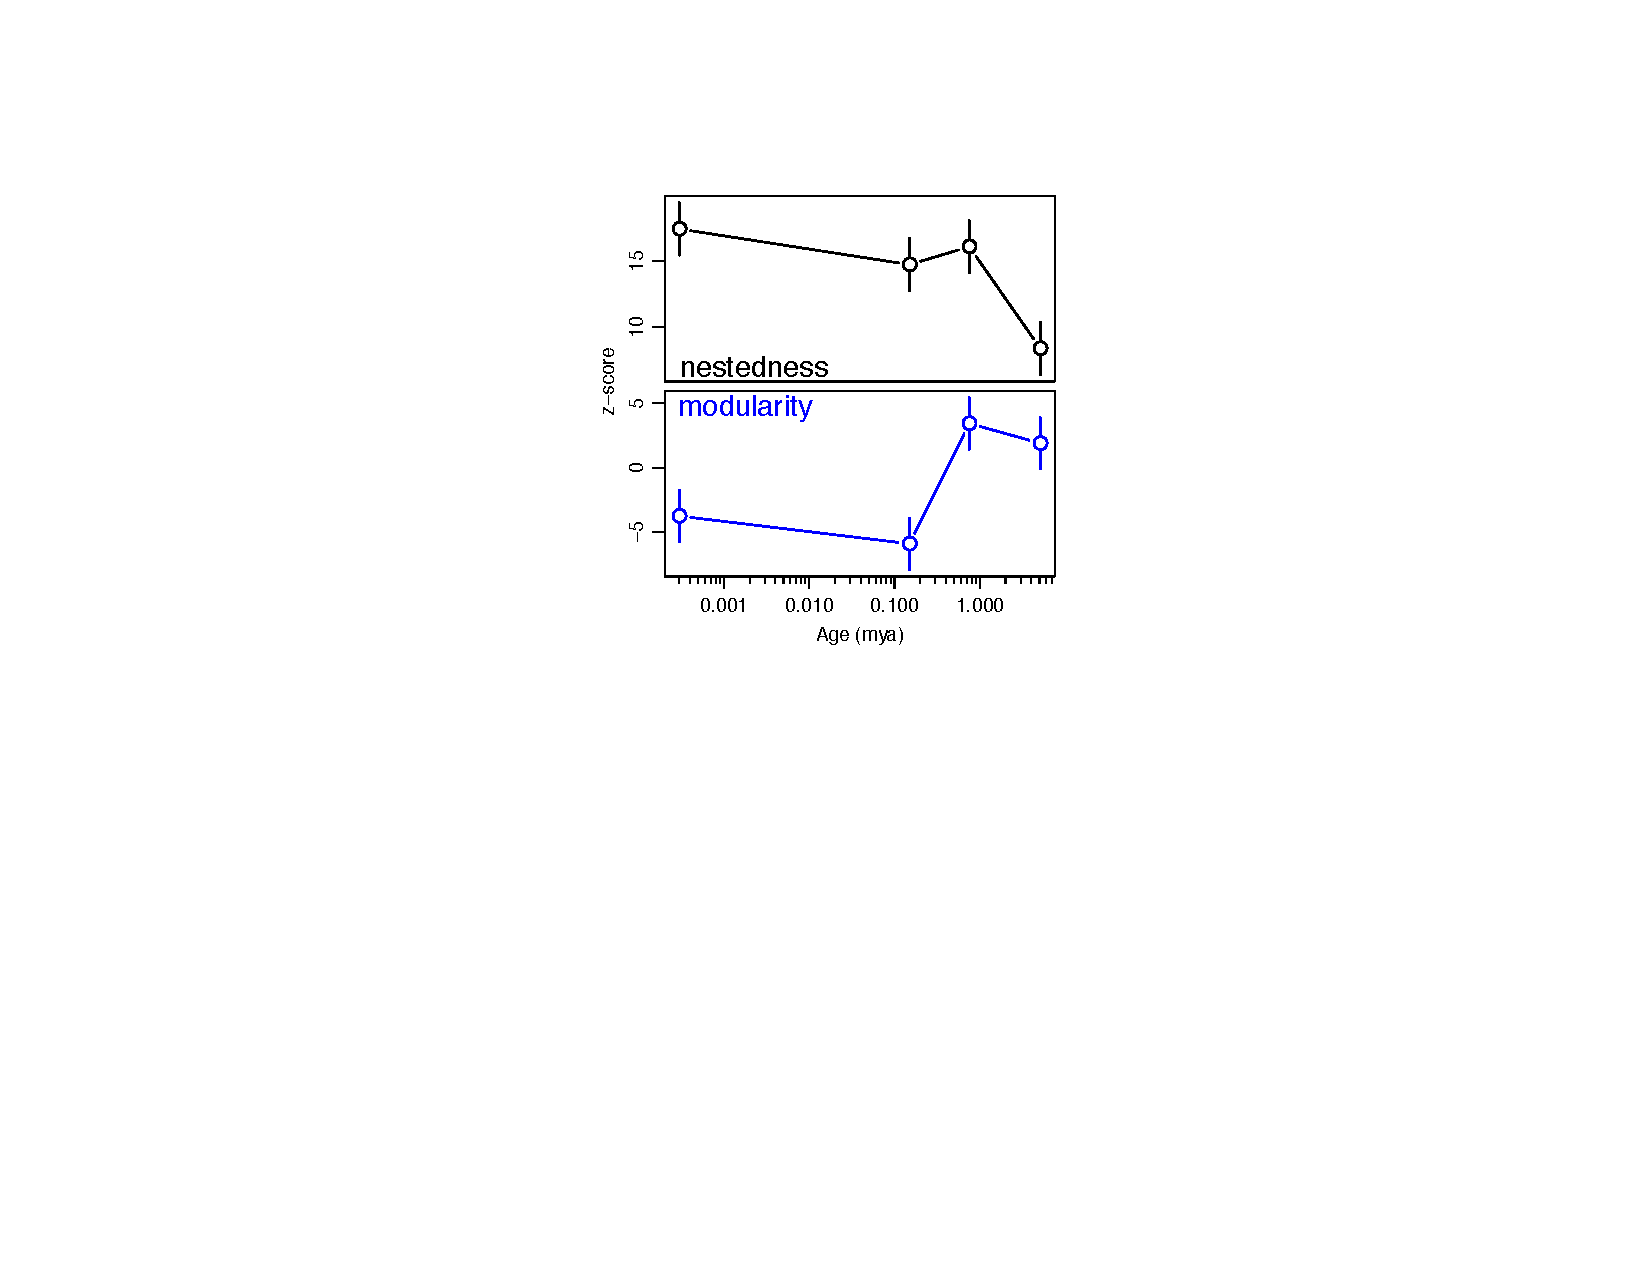
\includegraphics[scale=1]{fig_netMets.pdf} 
  \caption{Trends in network metric nestedness and modularity through
    time. Nestedness decreases while modularity increases. Error bars
    come from null model simulation. While sign of z-score depends on
    null model and method of calculating modules (see supplemental
    figure) overall trend is robust. Some level of nestedness is
    likely a statistical property of these networks, however it could
    also be driven by stabilizing ecological mechanisms. Modularity is
    thought to be a sign of coevolution driving convergence in traits
    of plants and herbivores. This very interesting peaks on Maui
    where adaptive diversification may be at its peak.}
  \label{fig:netMet}
\end{figure}


\begin{figure}[!hp]
  \centering
  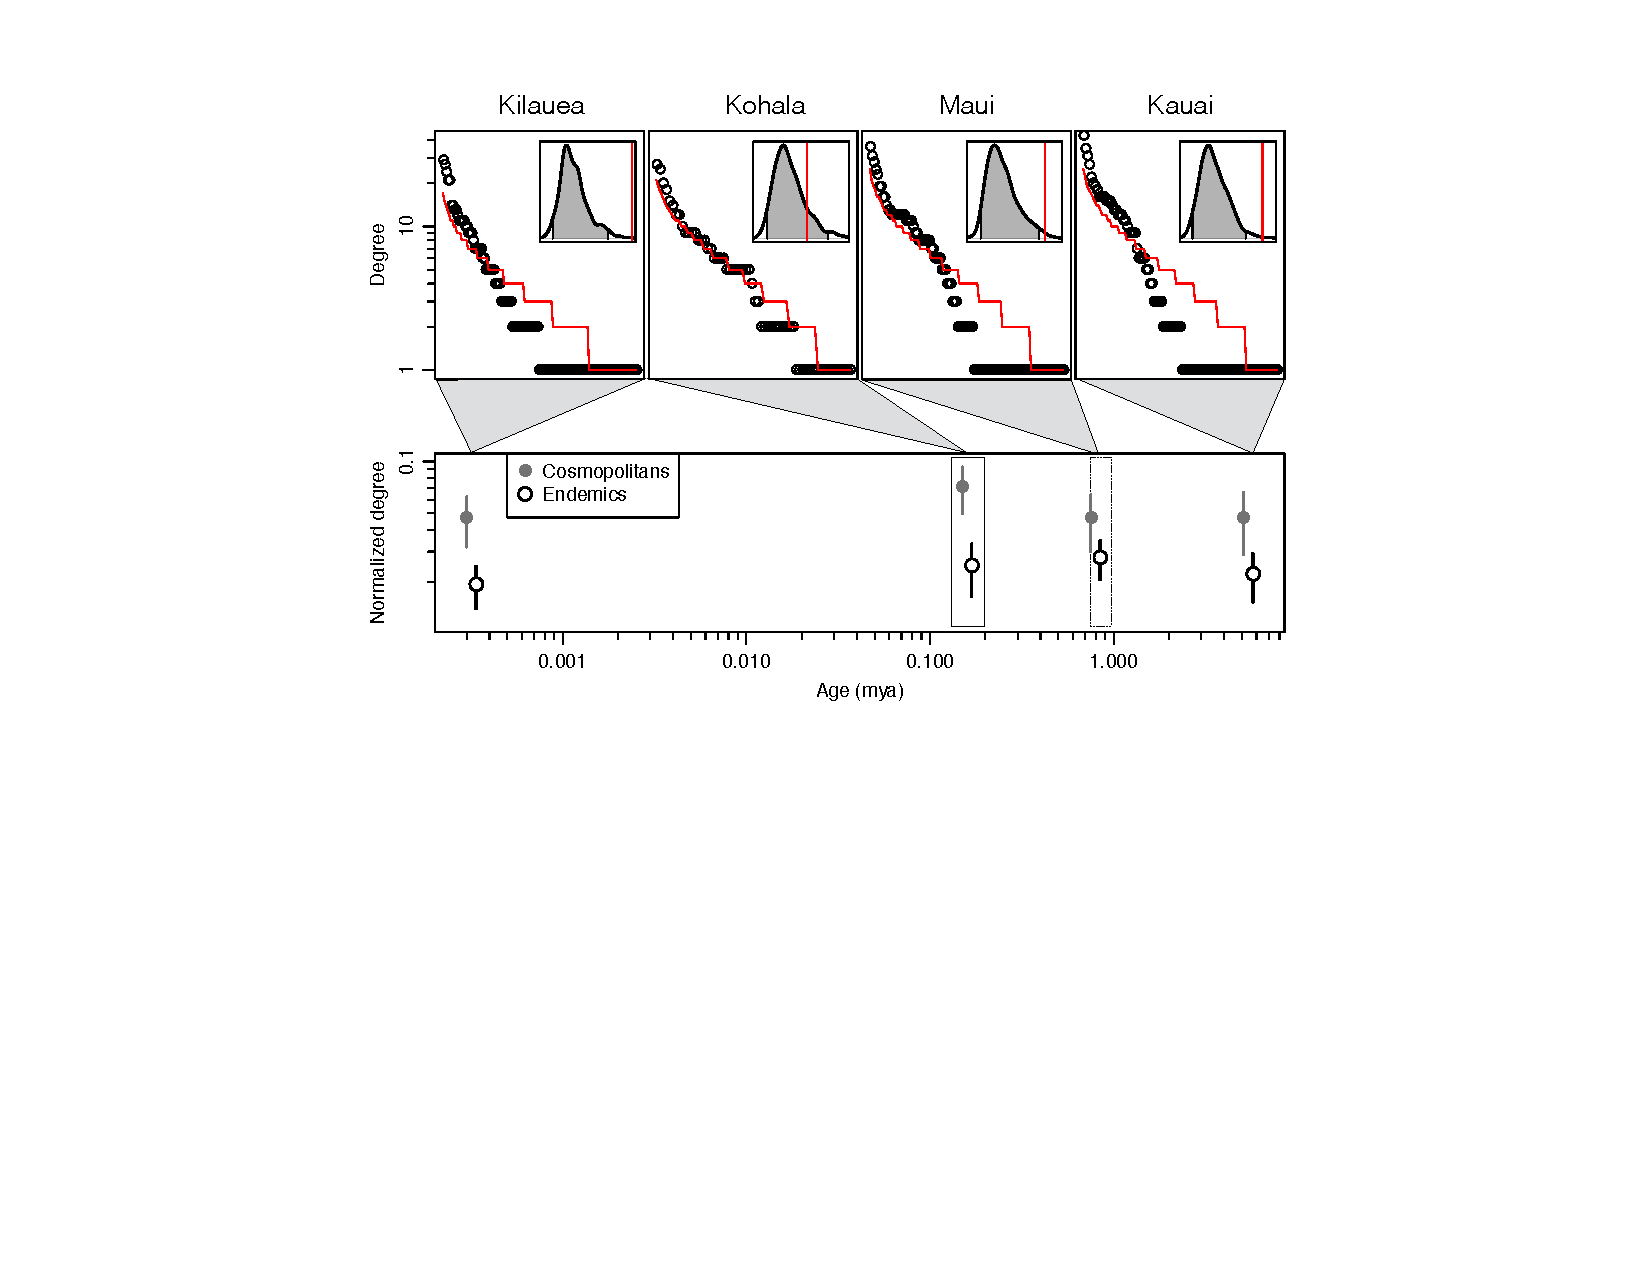
\includegraphics[scale=0.7]{fig_degree.pdf} 
  \caption{Patterns in degree distributions across sites and different
    biogeographic classifications of taxa. Top panels show that
    networks deviate most from MaxEnt on youngest and oldest
    sites. Deviation on Koh is not different than expected by
    chance. Koh shows minimal modularity, and maximal
    connectance. Bottom panel shows number of links for island
    endemics versus island cosmopolitans. Endemics show lower linkage
    overall, but significantly increase on the middle aged site
    Hal. Koh shows increased linkage overall. When looking at links to
    plant genera this pattern holds except that endemics on Hal no
    long show a difference in generality, indicating that the pattern
    is driven in part by plant diversity.}
  \label{fig:degree}
\end{figure}

\begin{figure}[!hp]
  \centering
  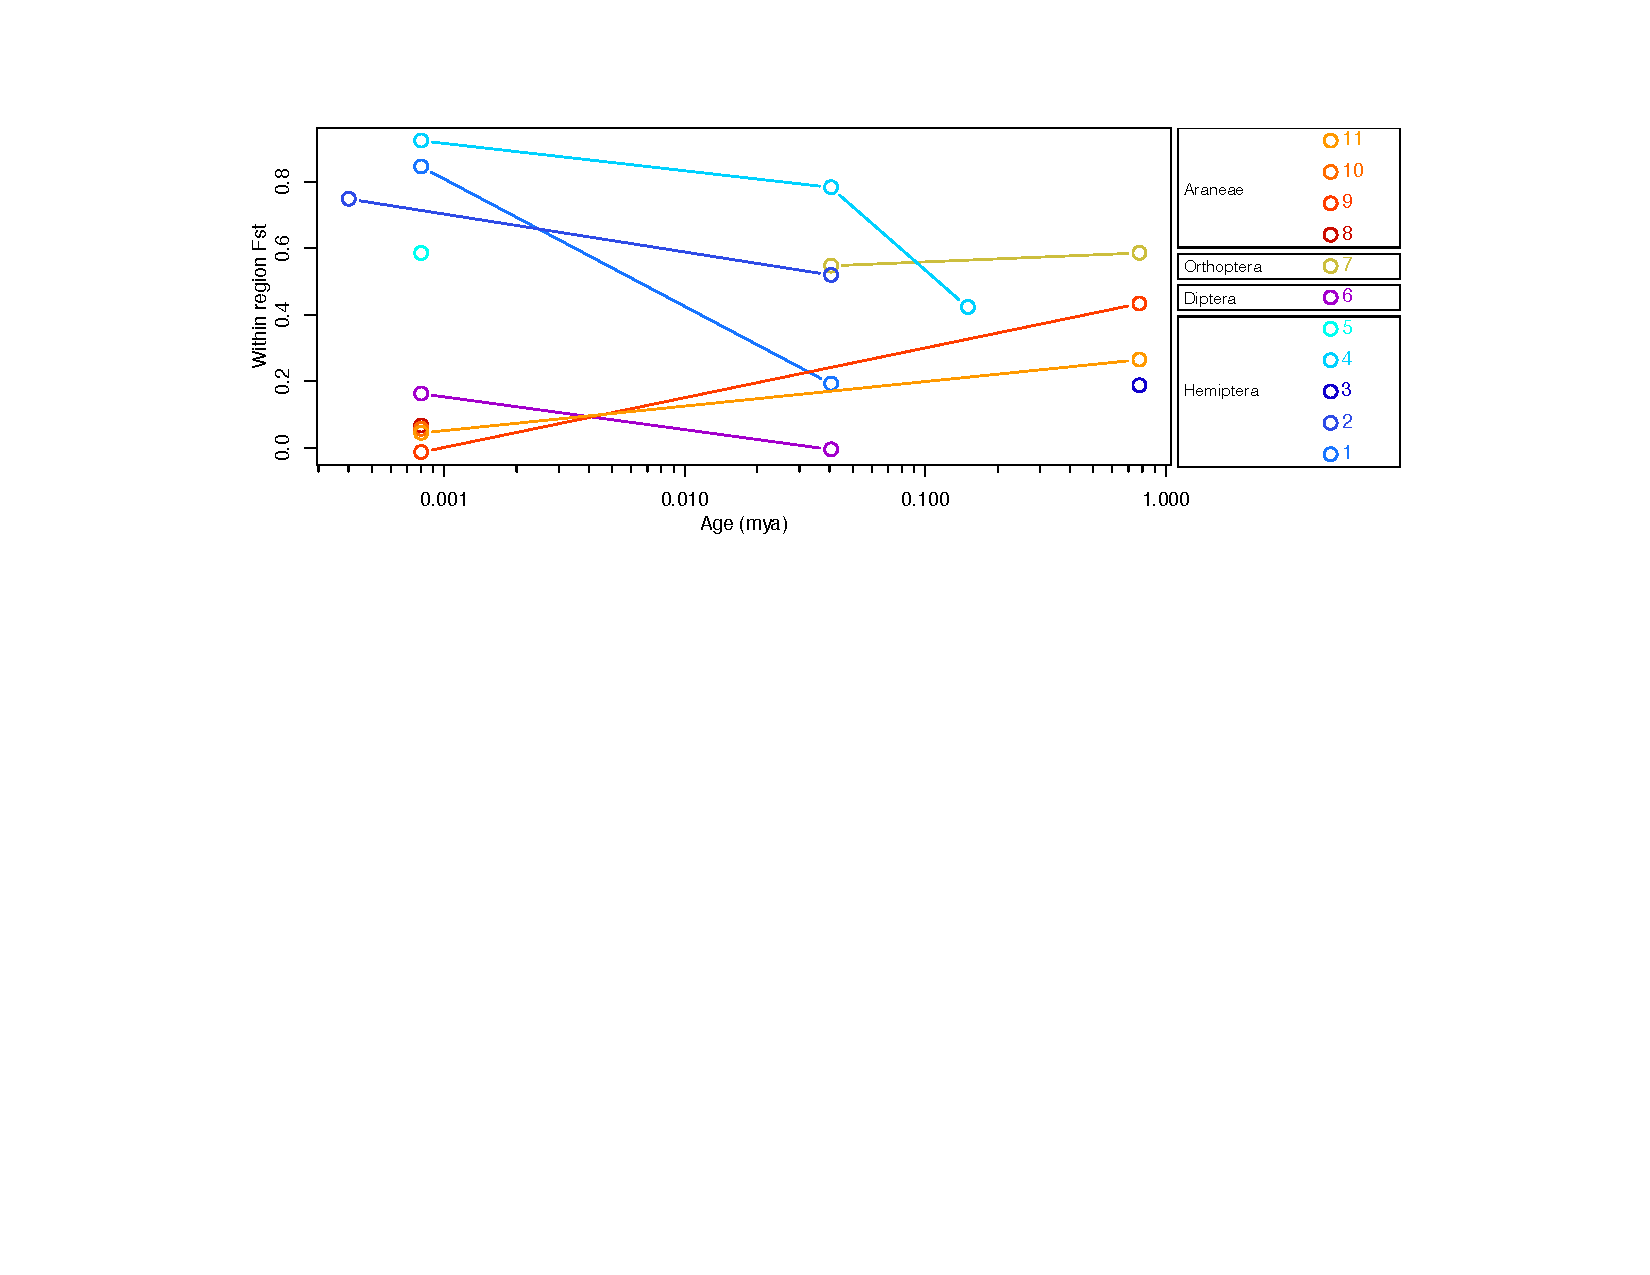
\includegraphics[scale=0.6]{fig_volcanoFst.pdf}
  \caption{Within volcano $F_{st}$ showing how volcano age influences
    this measure of structure and diversity.}
  \label{fig:volcanoFst}
\end{figure}

\clearpage

\section*{Tables}

\begin{table}[!htb]
  \centering
  \caption{Table of between volcano $F_{st}$, best viewed in dropbox
    right now.}
  \label{tab:fst}
\end{table}


\end{document}




















